\documentclass[a4paper,12pt,french]{article}

\usepackage[cours]{../../../Style}

\begin{document}

\title{Proportions, variations et pourcentages}
\date{}
\maketitle

\section{Proportions et pourcentages}

\subsection{Proportions}

\begin{prop}
Soit $E$ un ensemble non vide ayant un nombre fini d'éléments, et $A$ un sous-ensemble de $E$ ( $A \subset E$ ). On note respectivement $n_A$ et $n_E$ le nombre d'éléments de $A$ et $E$. La proportion d'éléments de $A$ dans $Ê$ est le nombre $p= \frac {n_A} {n_E}$.
\end{prop}

\begin{ex}

Dans une classe de Seconde comprenant 35 élèves, il y a 20 filles. La proportion de filles dans la classe est donc $p = \frac {20} {35} = \frac 4 7 \simeq 0.571$.

\end{ex}

\begin{rmq}
$p$ est un nombre compris entre 0 et 1. Il est parfois plus commode d'utiliser un pourcentage à la place. Pour cela, il suffit de décaler la virgule de deux rangs vers la droite.
\end{rmq}

\begin{ex}
Dans l'exemple précédent, la proportion de filles dans la classe est de $57.1 \%$.
\end{ex}

\rem{Attention avec les pourcentages: $0.5 = 50 \%$ et $7 \% = 0.07$}

\subsection{Proportions de proportions}

\begin{prop}
Soit $E$ un ensemble non vide ayant un nombre fini d'éléments, $A \subset E$ et $B \subset A$. On note $p_1$ la proportion de $A$ dans $E$ et $p_2$ la proportion de $B$ dans $A$. Alors la proportion de $B$ dans $E$ est égale à $p_1 \times p_2$.
\end{prop}

\begin{ex}
Dans l'exemple précédent, si $25 \%$ des filles portent des lunettes, alors la proportion de filles portant des lunettes dans la classe est $\frac {25} {100} \times \frac 4 7 = \frac 1 7 \simeq 0.142 = 14.2 \%$.
\end{ex}

\section{Evolutions et pourcentages}

\subsection{Taux d'évolution}

\begin{defin}
On considère une valeur $V_0$ qui subit une évolution pour arriver à une valeur $V_1$. \begin{itemize}
\item La variation absolue est $V_1 - V_0$.
\item La variation relative ou taux d'évolution est $t=\frac {V_1 - V_0} {V_0}$.
\end{itemize}
\end{defin}

\begin{rmq} \saut
\begin{itemize}
\item Si $t>0$, il s'agit d'une augmentation.
\item Si $t<0$, il s'agit d'une diminution.
\end{itemize}
\end{rmq} 

\begin{ex}
Le prix d'un article est passé de $150$ euros à $180$ euros. La variation absolue du prix est de $180-150=30$ euros et son taux d'évolution est $\frac {180-150}{150}=\frac{30}{150}=0.2=\frac{20}{100}$. Ce prix a donc subi une augmentation de $20 \%$.
\end{ex}

\begin{propr} Pour une valeur $V_0$ qui subit une évolution d'un taux $t$, elle devient $\left( 1+t \right) \times V_0$. \newline $1+t$ est appelé coefficient multiplicateur ( noté CM ).
\end{propr}

\begin{ex}
Le prix d'un abonnement à l'origine de $25$ euros augmente de $20 \%$. Il passe alors à $\left( 1 + \frac {20} {100} \right) \times 25 = 1.2 \times 25 = 30$ euros. Si le nouveau prix subit une diminution de $20 \%$, il passe à $\left( 1-0.2 \right) \times 30 = 24$ euros. 
\end{ex}

\subsection{Evolution réciproque} 

\begin{defin}
Une valeur $V_0$ subit une évolution de taux $t$ pour passer à $V_1$. On appelle évolution réciproque le taux $t'$ d'évolution de la valeur $V_1$ à la valeur $V_0$.
\end{defin}

\begin{prop}
Le coefficient multiplicateur de l'évolution réciproque est l'inverse de celui de l'évolution:

\hfill $CM'=\frac 1 {CM}$ \hfill
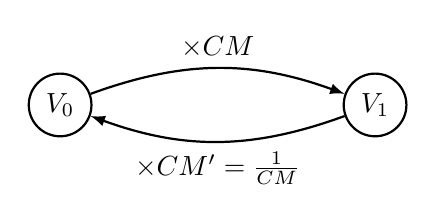
\begin{tikzpicture}[baseline=(current bounding box.center)]
\node[draw,circle,thick] (V0) at (-4,0) {$V_0$};
\node[draw,circle,thick] (V1) at (0,0) {$V_1$};
\draw[->,>=latex,thick] (V0) to[bend left=20] node[midway,above]{$\times CM$} (V1);
\draw[->,>=latex,thick] (V1) to[bend left=20] node[midway,below]{$\times CM'=\frac 1 {CM}$} (V0);
\end{tikzpicture}
\hfill \

\end{prop}

\begin{ex}
En un an, la population d'une ville a augmenté de $14 \%$ pour atteindre $4.56$ millions d'habitants. Elle a donc été multipliée par $1.14$. Le coefficient multiplicateur réciproque est $\frac 1 {1.14} \simeq 0.877$, ce qui correspond à une baisse de $12.3 \%$. L'an dernier, la ville possédait alors $4.56 \times 0.877 = 4$ millions d'habitants.

\begin{center}
\begin{tikzpicture}[scale=6]
\node[draw,ellipse,thick,minimum size=1.5cm] (V0) at (0,0) {$V_0=4$};
\node[draw,ellipse,thick,minimum size=1.5cm] (V1) at (1,0) {$V_1=4.56$};
\draw[->,>=latex,thick] (V0) to[bend left=20] node[midway,above]{$\times 1.14$} node[midway,below]{$+14 \%$} (V1);
\draw[->,>=latex,thick] (V1) to[bend left=20] node[midway,below]{$\times \frac 1 {1.14}=0.877$} node[midway,above]{$-12.3 \%$} (V0);
\end{tikzpicture}
\end{center}
\end{ex}

\subsection{Evolutions successives}

\begin{prop}
Si une évolution fait passer la valeur $V_0$ non nulle à la valeur $V_1$, et une seconde fait passer la valeur $V_1$ à la valeur $V_2$, alors l'évolution globale fait passer la valeur $V_0$ à la valeur $V_2$. Son coefficient multiplicateur est le produit des coefficients multiplicateurs.

\begin{center}
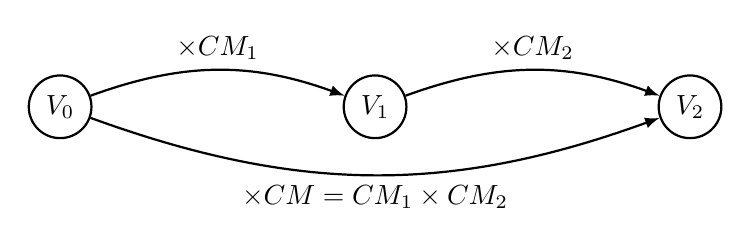
\begin{tikzpicture}
\node[draw,circle,thick] (V0) at (-4,0) {$V_0$};
\node[draw,circle,thick] (V1) at (0,0) {$V_1$};
\node[draw,circle,thick] (V2) at (4,0) {$V_2$};
\draw[->,>=latex,thick] (V0) to[bend left=20] node[midway,above]{$\times CM_1$} (V1);
\draw[->,>=latex,thick] (V1) to[bend left=20] node[midway,above]{$\times CM_2$} (V2);
\draw[->,>=latex,thick] (V0) to[bend right=20] node[midway,below]{$\times CM = CM_1 \times CM_2$} (V2);
\end{tikzpicture}
\end{center}
\end{prop}

\begin{ex}
Le prix d'un objet subit une hausse de $8 \%$ puis une nouvelle hausse de $10 \%$. Le coefficient multiplicateur global est donc $\left( 1+ \frac 8 {100} \right) \times \left( 1+ \frac {10} {100} \right) = 1.08 \times 1.1 = 1.188$. Le prix a donc augmenté de $18.8 \%$ et pas de $18 \%$ !
\end{ex}

\end{document}
